\documentclass[tikz]{standalone}
\usepackage{amsmath}
\definecolor{aksen}{RGB}{247,181,56}
\definecolor{bgdark}{HTML}{171D2B}
\begin{document}
\pagecolor{bgdark}
\color{white}
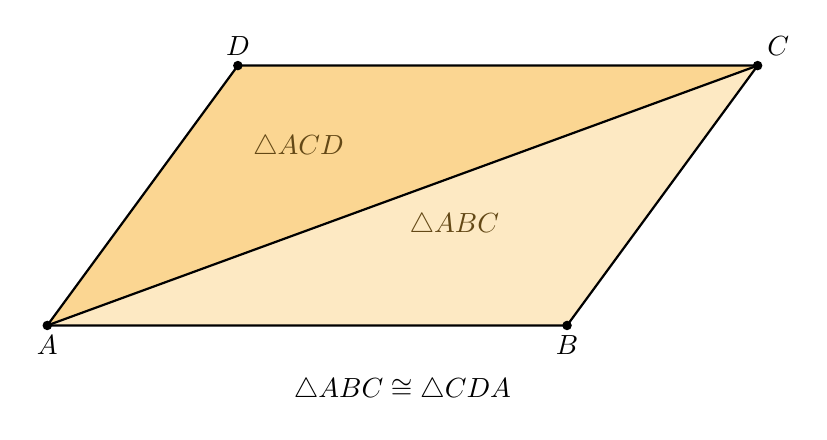
\begin{tikzpicture}[scale=1.1]
  % Panel 3: garis diagonal membagi jajargenjang jadi dua segitiga kongruen
  \begin{scope}
    \coordinate (A) at (0,0);
    \coordinate (B) at (6,0);
    \coordinate (C) at (8.2,3);
    \coordinate (D) at (2.2,3);
    \fill[color=aksen!30] (A) -- (B) -- (C) -- cycle;
    \fill[color=aksen!55] (A) -- (C) -- (D) -- cycle;
    \draw[thick] (A) -- (B) -- (C) -- (D) -- cycle;
    \draw[thick] (A) -- (C);
    \node[color=aksen!40!black] at (4.7,1.15) {$\triangle ABC$};
    \node[color=aksen!40!black] at (2.9,2.05) {$\triangle ACD$};
    \fill (A) circle (0.055) node[below] {$A$};
    \fill (B) circle (0.055) node[below] {$B$};
    \fill (C) circle (0.055) node[above right] {$C$};
    \fill (D) circle (0.055) node[above] {$D$};
    \node at (4.1,-0.75) {$\triangle ABC \cong \triangle CDA$};
  \end{scope}
\end{tikzpicture}
\end{document}
